%%%%%%%%%%%%%%%%%%%%%%%%%%%%%%%%%%%%%%%%%%%%%%%%%%%
%% P3: Phenomenology of Particle Physics                         
%%
%% Author:  André Rubbia                   		 
%%
%% Figure 6.1 Illustration of the transformation of a vector field under  a rotation.
%%
%% This work is licensed under the Creative Commons Attribution 4.0 International License. 
%% To view a copy of this license, visit http://creativecommons.org/licenses/by/4.0/ or 
%% send a letter to Creative Commons, PO Box 1866, Mountain View, CA 94042, USA.
%%
%%%%%%%%%%%%%%%%%%%%%%%%%%%%%%%%%%%%%%%%%%%%%%%%%%%

\documentclass[a4paper,10pt]{article}

\usepackage[T1]{fontenc}
\usepackage[utf8]{inputenc}
\usepackage{lmodern}
\usepackage[labelfont=bf]{caption}
\usepackage{upgreek}

\usepackage{tikz}
\usepackage{pgfplots}
\pgfplotsset{compat=1.17}
\usepgfplotslibrary{ternary}
\usepgfplotslibrary{fillbetween}
\usepgfplotslibrary{external}

\def\d{\mathrm{d}}

\begin{document}

%%%%%%%%%%%%%%%   FIGURE  %%%%%%%%%%%%%%%%%%%%%%%%%%%%%%
\begin{figure}[htb]
\begin{center}
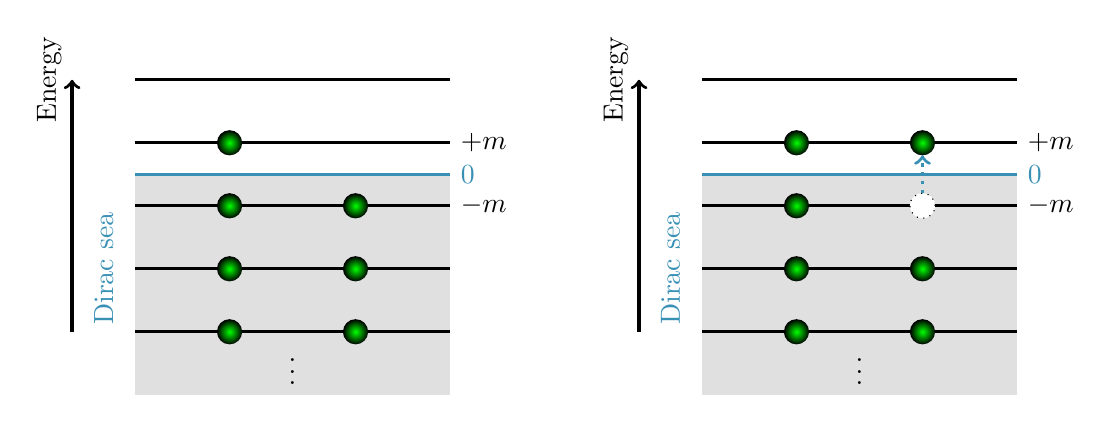
\begin{tikzpicture}[scale=0.8]
\begin{scope}[shift={(0,0)}]
\fill[fill=black!12!white] (0,-1) rectangle (5,2.5);
\draw[color=cyan!70!black,very thick] (0,2.5) -- +(0:5) node[right] {$0$};
\node[color=cyan!70!black,very thick,rotate=90] at (-0.5,1) {Dirac sea};
\draw[black,very thick,->] (-1,0) -- +(90:4) node[above,rotate=90] {Energy};
\draw[black,very thick] (0,0) -- +(0:5);
\draw[black,very thick] (0,1) -- +(0:5);
\draw[black,very thick] (0,2) -- +(0:5) node[right] {$-m$};
\draw[black,very thick] (0,3) -- +(0:5) node[right] {$+m$};
\draw[black,very thick] (0,4) -- +(0:5);
\node[color=black] at (2.5,-0.5) {$\vdots$};
\shade[inner color=green,outer color=black] (1.5,0) circle (0.2);
\shade[inner color=green,outer color=black] (3.5,0) circle (0.2);
\shade[inner color=green,outer color=black] (1.5,1) circle (0.2);
\shade[inner color=green,outer color=black] (3.5,1) circle (0.2);
\shade[inner color=green,outer color=black] (1.5,2) circle (0.2);
\shade[inner color=green,outer color=black] (3.5,2) circle (0.2);
\shade[inner color=green,outer color=black] (1.5,3) circle (0.2);
\end{scope}
\begin{scope}[shift={(9,0)}]
\fill[fill=black!12!white] (0,-1) rectangle (5,2.5);
\draw[color=cyan!70!black,very thick] (0,2.5) -- +(0:5) node[right] {$0$};
\node[color=cyan!70!black,very thick,rotate=90] at (-0.5,1) {Dirac sea};
\draw[black,very thick,->] (-1,0) -- +(90:4) node[above,rotate=90] {Energy};
\draw[black,very thick] (0,0) -- +(0:5);
\draw[black,very thick] (0,1) -- +(0:5);
\draw[black,very thick] (0,2) -- +(0:5) node[right] {$-m$};
\draw[black,very thick] (0,3) -- +(0:5) node[right] {$+m$};
\draw[black,very thick] (0,4) -- +(0:5);
\node[color=black] at (2.5,-0.5) {$\vdots$};
\shade[inner color=green,outer color=black] (1.5,0) circle (0.2);
\shade[inner color=green,outer color=black] (3.5,0) circle (0.2);
\shade[inner color=green,outer color=black] (1.5,1) circle (0.2);
\shade[inner color=green,outer color=black] (3.5,1) circle (0.2);
\shade[inner color=green,outer color=black] (1.5,2) circle (0.2);
%% hole
\shade[inner color=white,outer color=white] (3.5,2) circle (0.2);
\draw[dotted] (3.5,2) circle (0.2);
\shade[inner color=green,outer color=black] (1.5,3) circle (0.2);
\shade[inner color=green,outer color=black] (3.5,3) circle (0.2);
\draw[->, color=cyan!70!black,very thick,dotted] (3.5,2.2) -- (3.5,2.8);
\end{scope}
\end{tikzpicture}
\caption{Dirac hole theory: an electron with negative energy ``$-E$'' is
excited in a state with positive energy $E'>0$, leaving a hole in the sea.}
\label{fig:lochtheorie}
\end{center}
\end{figure}
%%%%%%%%%%%%%%%  END FIGURE  %%%%%%%%%%%%%%%%%%%%%%%%%%%%%%
%

\end{document}
